\documentclass[compress]{beamer}

\usepackage[utf8]{inputenc}
\usepackage{graphicx}
\usepackage{color}
\usepackage{colortbl}
\usepackage{listings}
\usepackage{caption}
\usepackage{pgfpages}
\usepackage{tabularx}
\usepackage{amsthm}
\usepackage{url}

%\usetheme[basergb={1,0.2,0.2}]{Dcon}
%\usetheme[baseRGB={23,102,34}]{Dcon}
\usetheme{Dcon} % default color

%%%%%%%%%%%%%%%%%%%%%%%%%%%%% Definitions %%%%%%%%%%%%%%%%%%%%%%%%%%%%%%%%%%%%%

\newcommand{\logounis}{
\begin{table}[h]
\centering
\begin{tabular}{ccc}

\includegraphics[width=.3\linewidth]{images/logos/lmu_logo} \hspace{0.3cm} &

\includegraphics[width=.3\linewidth]{images/logos/Uni_Aug_Logo_Basis_pos_A}
\hspace{0.3cm} &

\includegraphics[width=.3\linewidth]{images/logos/tum}
\end{tabular}
\end{table}}

\newcommand{\logose}{
\includegraphics[width=.2\linewidth]{images/logos/LogoSEengl}\hspace{5mm}}

\newcommand{\hl}[1]{\fcolorbox{red}{white}{#1}}
\newcommand{\todo}[1]{\hl{TODO: #1...}}
\newcommand{\review}[0]{\todo{REVIEW}}
\newcommand{\comm}[1]{\textsuperscript{\bf \color{red}{\tiny [#1]}}}
\newcommand{\q}[0]{\comm{?}}
\newcommand{\s}[0]{\comm{*}}

\newcommand{\scite}[1]{\textsuperscript{\tiny\cite{#1}}}

%\bibliographystyle{apalike}


\titlegraphic{\logounis}
\title[Visual Debugging for Robotics]
{A flexible visual framework\\ \strut for debugging complex robotic systems}
\subtitle{\scriptsize{Masters's Thesis in the Software Engineering Elite Graduate Program}}
\author[Felix Kaser]{Felix Kaser\\\tiny{\texttt{kaserf@in.tum.de}}}
%\institute[ISSE]
%{Institut für Software \& Systems \\
%Engineering}
\date{October 3, 2012}

\logo{\logose}

\additionaltext{\tiny
{Supervisors: Prof. Dr. Wolfgang Reif,\\
\hspace{20mm}Prof. Bruce A.~MacDonald, PhD.\\
\hspace{2mm}Advisor: M.Sc. Andreas Angerer}}

%%%%%%%%%%%%%%%%%%%%%%%%%%%%% Document %%%%%%%%%%%%%%%%%%%%%%%%%%%%%%%%%%%%%%%%%

\begin{document}

% title page
\begin{frame}[plain]
\titlepage
\end{frame}

\begin{frame}{Outline}
\tableofcontents
\end{frame}

\section{Introduction}
%%%%%%%%%%%%%%% Introduction %%%%%%%%%%%%%%%%%%%%%%%
\subsection{Problem Statement}

\begin{frame}{Problem Statement}
\begin{itemize}
\item Debugging in robotics is complex
\item Traditional debugging tools lack support for robotics
\item Specialized tools are needed to cope with the requirements of robotics
\end{itemize}
\pause
\textbf{Key problems:}
\begin{itemize}
\item Robotic applications are usually not interruptible
\item The data handled in robotic systems comes from sensors instead of user-input
\item Data is hard to understand in its raw form
\item The robotics field is diverse and tools are often created for really specific use cases and cannot be easily re-used
\end{itemize}
\end{frame}

\begin{frame}{Hypothesis}
\begin{block}{}
A visualization tool for robotics that allows developers to choose the visualization they prefer can reduce the cognitive load during debugging and thus improve development speed.
\end{block}
\end{frame}

\subsection{Debugging in Robotics}

\begin{frame}{Related Tools}
\begin{itemize}
\item Realtime Debugging
\item National Instruments LabVIEW
\item Augmented Reality (AR) Debugging
\end{itemize}
\end{frame}

\begin{frame}{Realtime Debugging}
\begin{columns}
\begin{column}{.5\textwidth}
\begin{itemize}
\item Developed by Luke Gumbley at the robotics lab
\item Extends GDB to support realtime data collection
\item Integrated into NetBeans IDE
\end{itemize}
\end{column}
\hfill%
\begin{column}{.5\textwidth}
\begin{figure}[htbp]
  \centering
  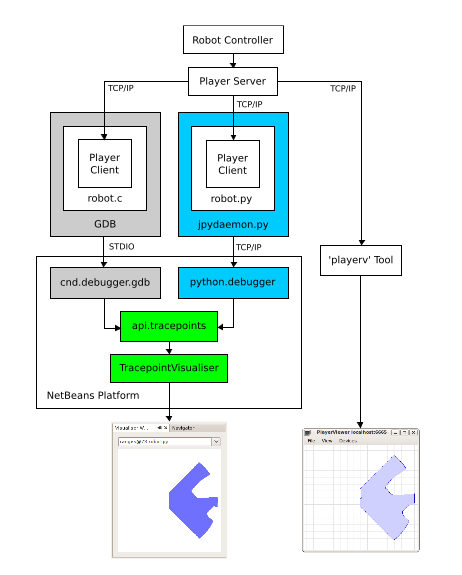
\includegraphics[width=.75\textwidth]{images/tracepoints_gumbley.png}
  \caption{Tracepoints block diagram. \cite{Gumbley2009}}
\end{figure}
\end{column}
\end{columns}
\end{frame}

\begin{frame}{LabVIEW}
\begin{itemize}
\item Graphical programming tool developed by National Instruments
\item Front panels allow to create specific user interfaces for the program
\item Front panels are connected in the visual program
\end{itemize}
\end{frame}

\begin{frame}{LabVIEW}
% source: public domain image from http://en.wikipedia.org/wiki/File:WikipediaFPandBD.png
\begin{figure}[htbp]
  \centering
  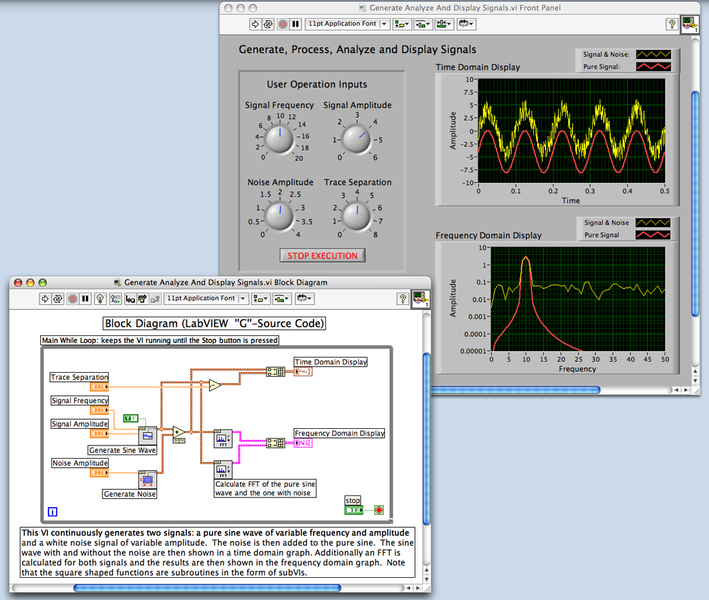
\includegraphics[width=.6\textwidth]{images/labview_frontpanel.png}
  \caption{Screenshot of the LabVIEW user interface with front panels in the top right.}
\end{figure}
\end{frame}

\begin{frame}{AR Dev}
\begin{itemize}
\item Realtime Debugging \cite{Gumbley2009}
\item National Instruments LabVIEW
\item Augmented Reality (AR) Debugging \cite{Collett2010}
\end{itemize}
\end{frame}

\begin{frame}{Problems of Existing Tools}
\begin{itemize}
\item High configuration overhead
\item Visualization focuses on pre defined data
\item Arbitrary data is usually rendered as text
\end{itemize}
\end{frame}

\section{ROS (Robot Operating System)}

\subsection{Overview}
\begin{frame}{Overview}

\begin{columns}
\begin{column}{.6\textwidth}
%left column
\begin{itemize}
\item Developed first at Stanford, now at Willow Garage
\item Modular robotic middleware
\item Active open source community
\item Many ready to use solutions for common problems in robotics (SLAM, transformations, grasping, ...)
\end{itemize}
\end{column}%
\hfill%
\begin{column}{.48\textwidth}
%right column
\begin{figure}[t]
    \centering
    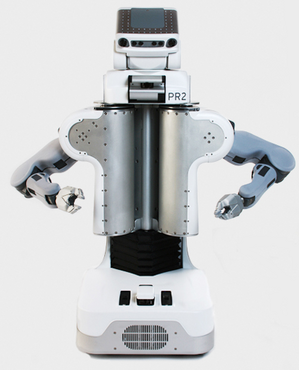
\includegraphics[width=0.7\textwidth]{images/pr2.png}
    \caption[The PR2 robot]{The PR2 robot}
\end{figure}
\end{column}%
\end{columns}
\end{frame}

%\subsection{ROS Basics}
\begin{frame}{ROS Basics}
\begin{itemize}
\item Modules are called nodes
\item Communication infrastructure based on publish/subscribe
\end{itemize}
\pause
\begin{block}{Publish/Subscribe:}
explain pubsub
\end{block}
\end{frame}

\subsection{Existing ROS Tools}
\begin{frame}{Existing ROS Tools}

\begin{columns}
\begin{column}{.3\textwidth}
%first column
RViz
\end{column}%
\hfill%
\begin{column}{.3\textwidth}
%second column
rxconsole
\begin{figure}[t]
    \centering
    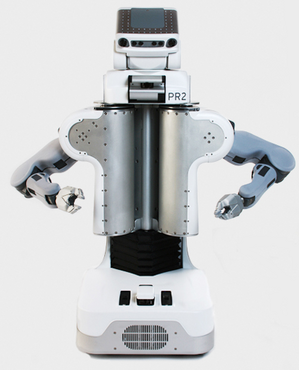
\includegraphics[width=0.7\textwidth]{images/pr2.png}
    \caption[The PR2 robot]{The PR2 robot}
\end{figure}
\end{column}%
\hfill%
\begin{column}{.3\textwidth}
%third column
rxbag
\end{column}
\end{columns}
\end{frame}

%\subsection{Logging in ROS}
\begin{frame}{Logging in ROS}
\begin{itemize}
\item C++ and Python client libraries contain logging API
\item Log messages are sent to console, log file and \emph{/rosout}
\item Can be filtered by severity and text
\item Log messages are text only with metadata (timestamp)
\end{itemize}
\end{frame}

\section{ROSDashboard}
%%%%%%%%%%%%%%%% ROSDashboard section %%%%%%%%%%%%%%%%%%%
\subsection{Goals}

\begin{frame}{Goals}
\begin{itemize}
\item Create a easy to use debugging tool
\item Visualize simple and abstract data
\item Allow developers to choose the visualization they prefer
\item Extendible through plugins
\item Create a tool to evaluate hypothesis
\end{itemize}
\end{frame}

\subsection{Requirements}
\begin{frame}{Requirements}
\begin{itemize}
\item Distributed live debugging
\item Transparent connection to data collection
\item Adaptability to different preferences and use cases
\item Low configuration overhead to keep developer on task
\end{itemize}
\end{frame}

\subsection{Design}

\begin{frame}{System Design}
\begin{itemize}
\item Make use of ROS topics for transparent access to data
\item Flexible and configurable user interface
\item Visualizations wrapped in widgets
\item Framework that allows easy integration of a plugin system
\end{itemize}
\end{frame}

\begin{frame}{Object Design}
\begin{figure}
    \centering
    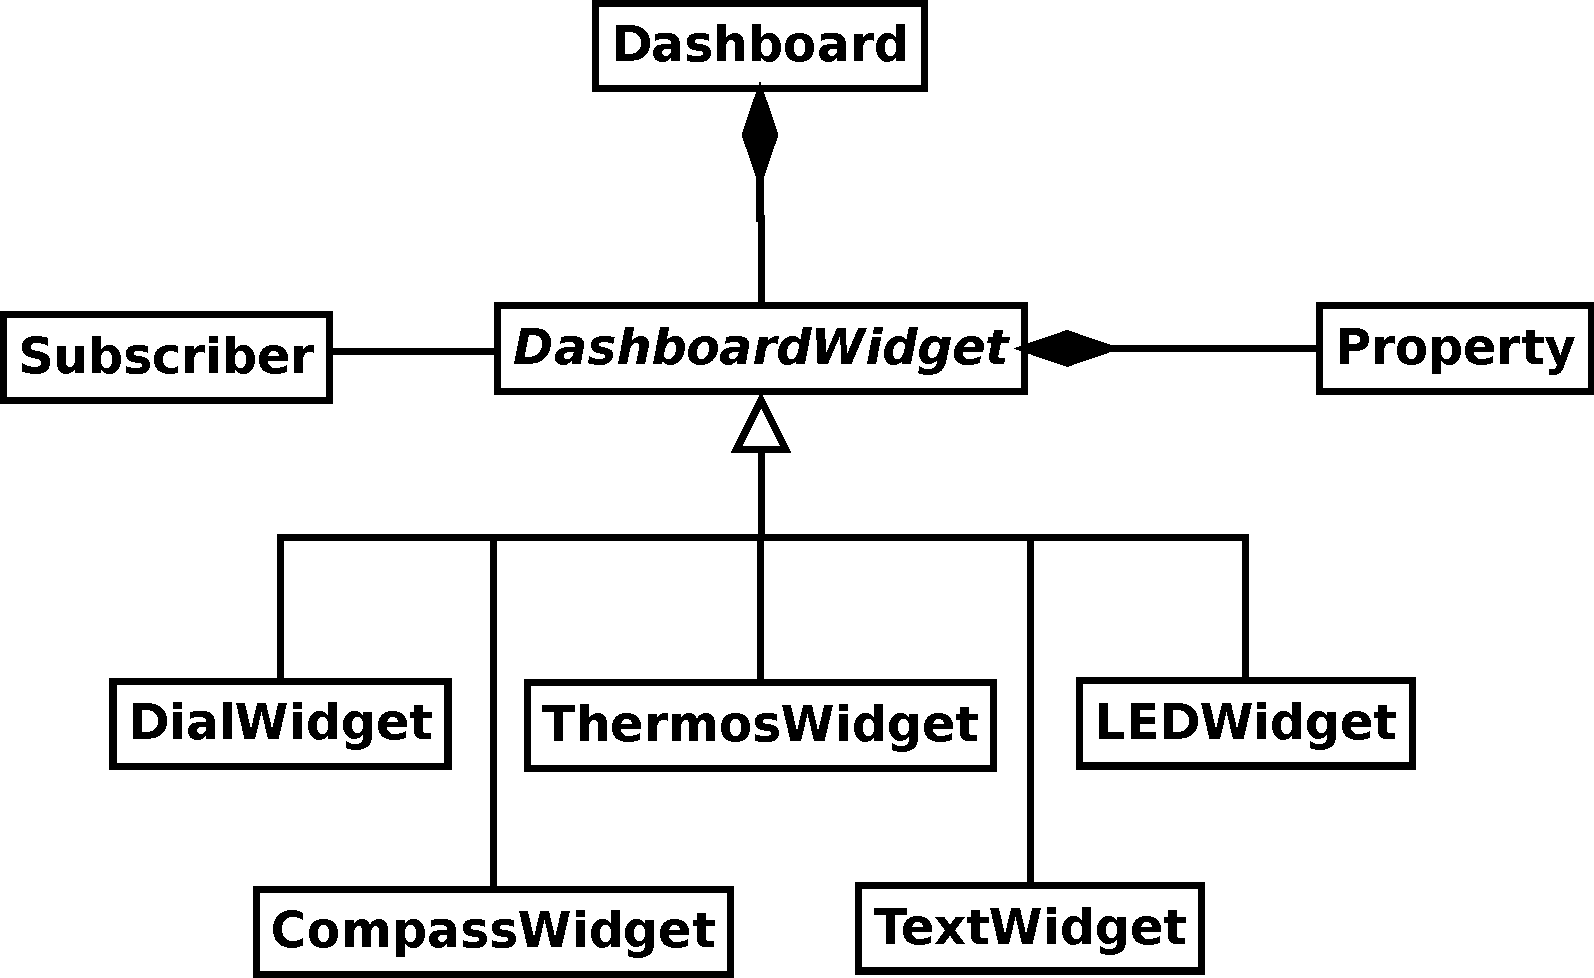
\includegraphics[width=0.7\textwidth]{diagrams/class_overview}
    \caption[Core object model overview]{Core object model overview}
\end{figure}
\end{frame}

%\begin{frame}{Global Control Flow}
%\begin{figure}
%    \centering
%    \includegraphics[width=\textwidth]{../latex/diagrams/global_control_flow_new.pdf}
%    \caption{The Global Control Flow through the Subsystems (UML sequence diagram)}
%\end{figure}
%\end{frame}

\section{Outlook}

\subsection{Conclusion}

\begin{frame}
\begin{center}
\huge
Thanks for the attention
\end{center}
\end{frame}

\subsection{Future Work}

\begin{frame}
\begin{center}
\huge
Thanks for the attention
\end{center}
\end{frame}

\subsection{Thanks}

\begin{frame}
\begin{center}
\huge
Thanks for the attention
\end{center}
\end{frame}

\appendix
\pagenumbering{Roman}

%%%%%%%%%%%%%%%%%%%%%%%%%%%%%%%%% Appendix %%%%%%%%%%%%%%%%%%%%%%%%%%%%%%%%%%%%%%%%%%

\section{Bibliography}
\begin{frame}[allowframebreaks]{Literature}
\bibliographystyle{unsrt}
\bibliography{../latex/bibtex/Master_Thesis,../latex/bibtex/manual}
\end{frame}

%\section{Additional Material}
%\begin{frame}{Use Case Overview}
%\begin{figure}
%    \centering
%    \includegraphics[height=0.7\textheight]{../latex/diagrams/use_cases_overall.pdf}
%    \caption{Overall use case diagram (UML use case diagram)}
%\end{figure}
%\end{frame}

%\begin{frame}[allowframebreaks]{Object Design}
%\begin{figure}
%    \centering
%    \includegraphics[height=0.5\textheight]{../latex/diagrams/InteractionPatterns.pdf}
%    \caption{Matching Interactions to InteractionPatterns (UML class diagram)}
%\end{figure}

\end{document}
